\section{Desynthesis Attack}

An implicit assumption made in existing locking locking schemes is that a scheme is secure as long as the foundry has no access to an activated chip \emph{or} to designer-provided test-patterns\cite{plaza2015solving}. Roy et al., as a matter of fact, assert in their original paper, that an XOR-locked netlist ``gives no criterion to check for possible [common keys]"\cite{}.  In this section, we show that this is not the case; that in fact, an XOR-locked netlist contains significant information about the IP holder's common key, and that as such, neither XOR locking or any of the other XOR-based existing locking schemes; should be considered secure.

To do so, we describe an attack procedure that --- given only a locked netlist, and \emph{no input-output behavioural information} --- manages to recover a significant portion  (up to 88\%) of the common key bits, both when XOR locking and interference-based locking are used to lock a common collection of digital design benchmarks, the MCNC benchmark set~\cite{}. 

We start by demonstrating our attack using a simple example, the circuit in Figure \ref{}. Suppose the designer starts with this circuit as a behavioral description for some (simple) functionality to be implemented. Running Encounter RTL compiler --- a widely-used \cite{} commercial tool for logic synthesis --- on such a description results in the implementation shown in Figure \ref{}. Now suppose the implementation is XOR-locked prior to physical design (in the manner described by Roy et al.); in order to protect the design from overbuilding by the fab. This consequently results in the netlist in Figure \ref{} --- where, after inserting the two key gates, we moved inverter corresponding to key bit $k_1$ up and down the netlist (supposedly to conceal the fact that $k_1$'s correct value is $1$).

\begin{figure}%{L}{0.42\columnwidth}
\centering
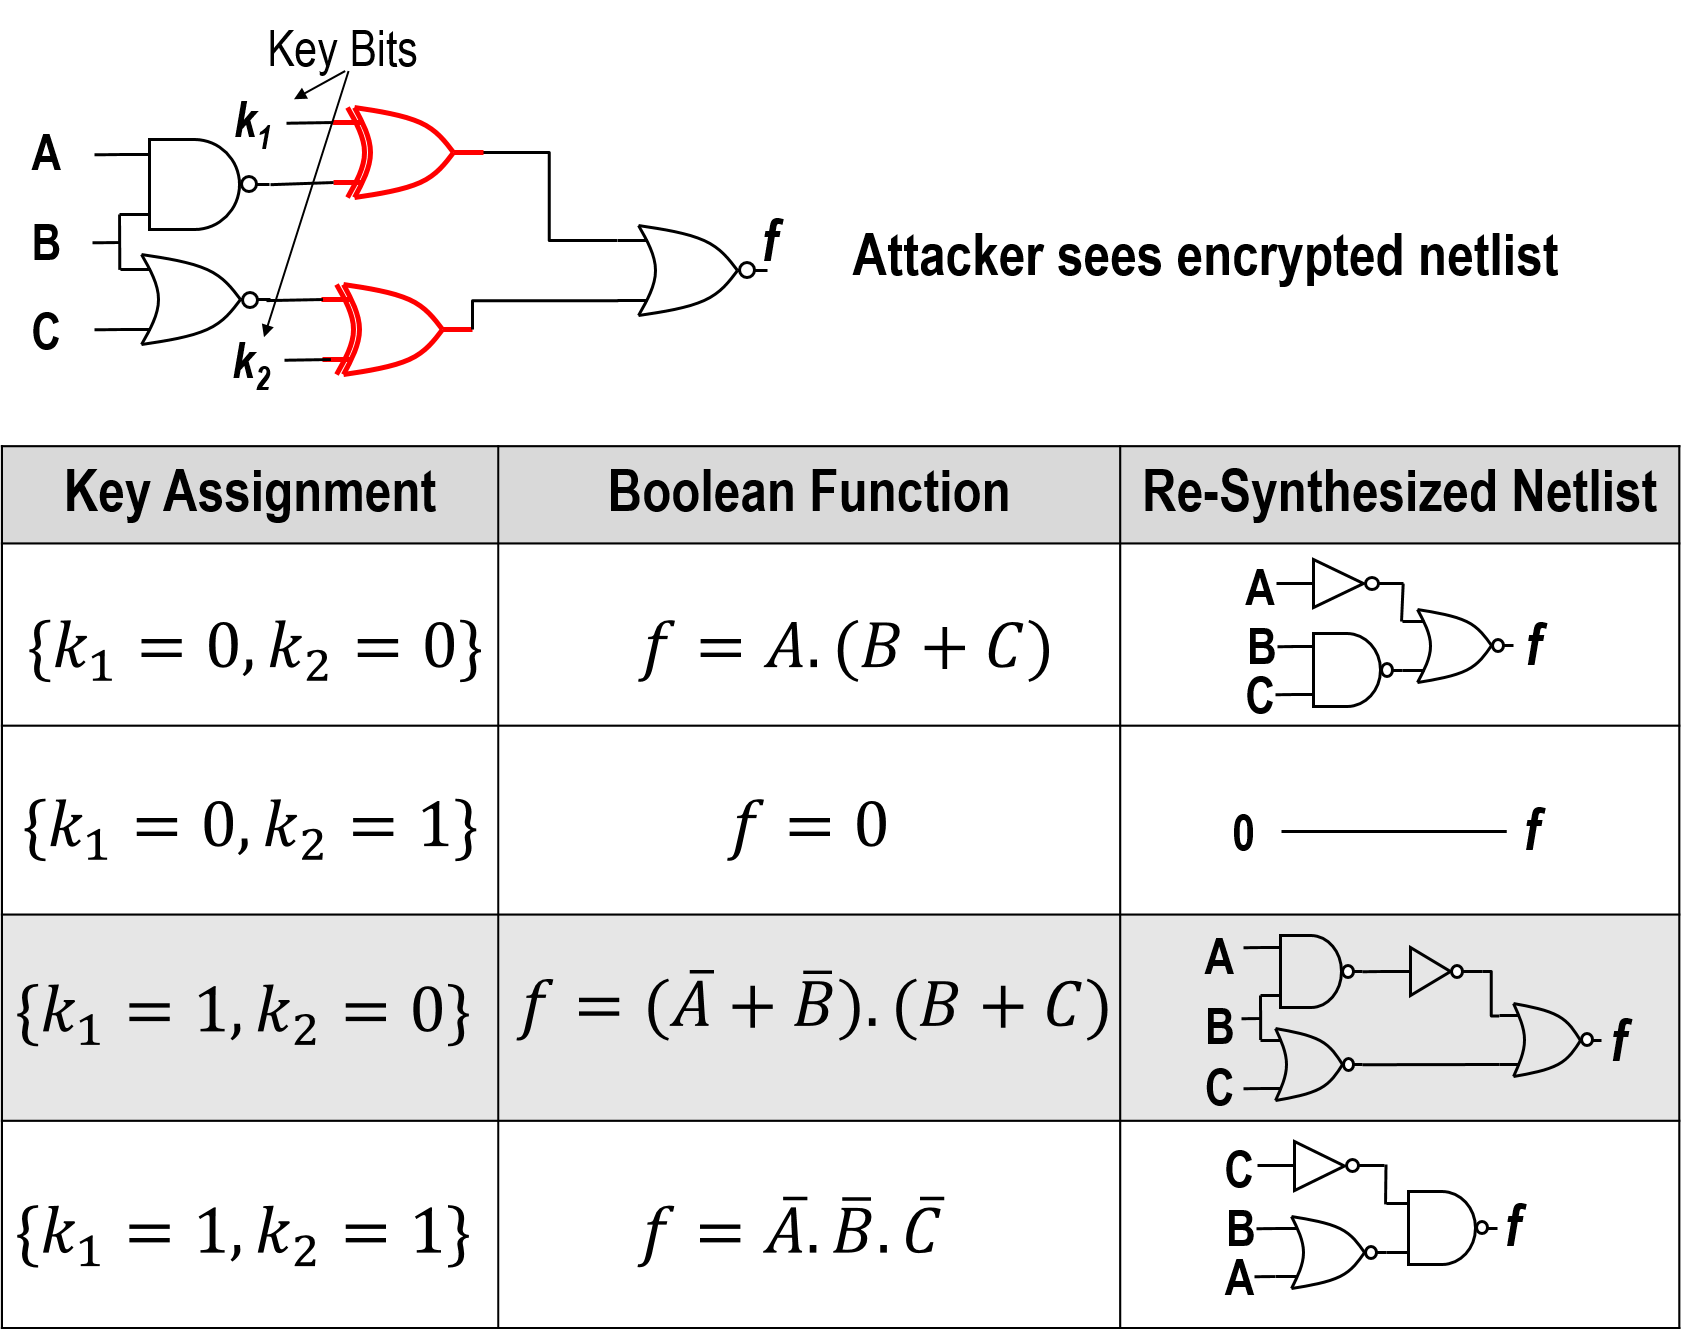
\includegraphics[width=0.9\columnwidth]{./figs/desynth.png}
\caption{An illustration of the desynthesis attack on the encrypted netlist from Figure~\ref{fig:lenc}. 
%All but the correct key result in netlists with fewer gates and different structure compared to the encrypted netlist (minus key gates) that the untrusted foundry sees.
}
\label{fig:desynth}
\end{figure}

Consider now each of the four possible key combinations, listed in Figure \ref{}; side-by-side with four netlists that we generated as follows. For each key combination, we take the locked netlist and set the key gate inputs to their respective values. We then replace each gate in the resulting netist was with a logic node of equivalent logic function, and re-map the resulting network (using, again, Encounter RTL compiler). This results in four (distinct) netlists in the figure, of which we make the following two observations:

\begin{enumerate}
    \item Out of the four netlists, only the one corresponding to the correct key has the same topology as the locked netlist (modulo inverters, CK inputs and key gates).
    \item Each of the netlists corresponding to the three incorrect key combinations has fewer gates that the locked netlist (even when key gates are disregarded)
\end{enumerate}

It appears that in this case, one can make the claim that \emph{synthesizing a network of equivalent Boolean function to the unlocked netlist (using the same synthesis tool that was used by the IP holder) --- results in a netlist that is similar, \emph{in structure}, to the locked one}. Our conjecture that the same holds for a wide class of circuits and synthesis tools forms the premise for our attack.

\paragraph{Attack Procedure} Our attack works by observing the differences between the resynthesized \footnote{We use the term resynthesis to refer to the process of ``erasing" the mapping of a technology-mapped network (by replacing each gate with a logic node of equivalent function); followed by a round of mapping transformations.} netlist corresponding to a candidate key value, and the (locked) netlist which the fab receives from the IP rights holder; then uses this information to guide a search for the  common key of the IP holder. If a designer chooses a long enough common key, an exhaustive search for the key is naturally out of the question. So we instead performs a \emph{local} search: starting with a random guess for the common key, we iteratively improve upon the guess by exploring the immediate neighbourhood of keys, looking for key values with corresponding resynthesized netlists that better match the one that the fab sees (according to some difference metric). To better explore the key space, and to decrease the chances of hitting a less than optimal local minima, we perform the local search multiple times, each time start with a different initial key guess. The attack algorithm is shown as Algorithm \ref{attack_alg}. In the algorithm, resynthesize() takes a locked netlist and a key guess and returns the resynthesized netlist corresponding to the key guess. Difference() is a function that takes two --- locked and unlocked --- netlists and returns the value of the difference metric. 

%\floatname{algorithm}{Procedure}
\renewcommand{\algorithmicrequire}{\textbf{Input:}}
\renewcommand{\algorithmicensure}{\textbf{Output:}}

\begin{algorithm}
\caption{Desynthesis Attack}
\label{attack_alg}
\begin{algorithmic}
\REQUIRE A locked netlist $N$ and the number of restarts for the local search $restarts$
\ENSURE A guess, $ck$, for the value of the common key that was used to generate $N$
\STATE{$key\_size\leftarrow $number of key bits in N}
\STATE $abs\_min \leftarrow INF$
\FOR{$i=1$ \TO $restarts$}
\STATE $guess \leftarrow $a random bitstring of size $key\_size$
\WHILE{\TRUE}
%\STATE $min=0$
\STATE $bit=-1$
\STATE{$N1 \leftarrow \textnormal{resynthesize}(N,guess)$}
\STATE{$min\leftarrow \textnormal{difference}(N1,N)$}
\FOR{$j=1$ \TO $key\_size$}
\STATE{Toggle $j^{\textnormal{th}}$ bit of $guess$}
\STATE{$N1 \leftarrow $resynthesize$(N,guess)$}
\STATE{$diff\leftarrow $difference$(N1,N)$}

\IF{$diff<min$}
\STATE{$min=diff$}
\STATE{$bit=j$}
\ENDIF
\STATE{Toggle (back) $j^{\textnormal{th}}$ bit of $guess$}
\ENDFOR
\IF{$bit=-1$}
\STATE{break}
\ELSE
\STATE{Toggle (again) $bit^{\textnormal{th}}$ bit of $guess$}
\ENDIF
\ENDWHILE
\IF{$min<abs\_min$}
\STATE{$best\_guess=guess$}
\STATE{$abs\_min=min$}
\ENDIF
\ENDFOR
\RETURN $best\_guess$
\end{algorithmic}
\end{algorithm}

Figure \ref{} shows the attack results for the scf benchmark from the MCNC benchmark set~\cite{}, when the benchmark is synthesized using the ABCsynthesis tool, and the netlist is locked using the XOR locking algorithm, with keys of size 32, 64, and 128. T

%The fab can use a variety of difference metrics. We experimented with  By using \emph{very} simple metrics for the difference between netlists (we model netlists as colored directed acyclic graphs), 

We observe that the algorithm recovers a significant portion of the key bits, for (and for keys long enough to make an exaustive search infeasible) . We report the attack results for other benchmarks in the MCNC set in Section ??.

(we report results of statistical significance tests against this hypothesis in Section ??)
%that It Looking at each of the four netlists, and knowing the locking scheme that the designer used to lock the cir --- the structural . 

So clearly, and contrary to the claim in \cite{roy2008epic}, the locked netlist here \emph{does} offer some criteria to check for possible common keys. Had locked netlists indeed lived up to this claim, we should be able to recover no more that 50\% of the key bits, on average, for \emph{every} design that we throw at the locking scheme .

%Now consider the following algorithm for deducing the common key from a locked netlist. The attacker starts with a random key guess. They then perform a hillIn Section xxxx, we describe a concrete attack procedure, that --- for all benchmarks in the MCNC benchmark set --- manages to recover xxxx , when the benchmarks are locked using both Igor's \cite{} and JV's \cite{} schemes. The success of the attack in recovering indicates that both schemes introduce significant information about the IP holder's common key in locked netlists, and as such must not be considered secure. 
%therefore a netlist locked according to both schemes does offer some criterion to check for possible common key combinations, contrary to the claims in \cite{}.

\paragraph{What are existing locking schemes doing wrong?} A quick look at published locking schemes reveals a trend to perform locking on some form of technology-mapped netlist (\cite{} and \cite{}), or unspecified (but implied to be a network, as in \cite{}), in contrast to performing the locking modifications on the RTL. To some extent, this is justifiable. For a start, one can argue that it is easier to lock a network representation of a circuit; as opposed to an abstract form of desired behaviour (as might be said of Verilog or VHDL code). To see this, consider that a Boolean network typically offers more room for modifications by a locking algorithm than would be available in an initial RTL description (e.g., a single Verilog line of code such as z = a + b where a and b are 32-bit registers will be converted by a Verilog compiler to a network with at least 32 XOR gates, each of which offers a candidate location for locking, e.g. by inserting a key gate at the output). 

The second correctness criterion is also easier to satisfy when working on Boolean network rather than RTL. For example in the context of XOR locking, one can use an automatic test pattern generation tool to make sure that two stuck-at-faults at the selected wires do not cancel each other out, thereby rendering some incorrect key equivalent to the correct one, in the sense that applying the incorrect key results in correct circuit behaviour. Given that ATPG tools accept netlists as input, it is attractive to defer locking till at least some form of synthesis has been performed (e.g, until a corresponding multi-level network has been constructed by the synthesis tool, as a first step to prepare the network for optimization).

%In this paper, we argue that

Unfortunately, while convenient, performing locking post-synthesis (or in general, after some optimizing transformation has been applied on the RTL) in a logic locking scheme, nonetheless introduces a subtle (fundamental?) --- yet significant --- vulnerability in the scheme, %the one we exploit in our attack procedure. 
This vulnerability comes about as a result of the fact that --- Unlike ``raw" RTL (pre-synthesis) --- in an optimized network, different parts of the network are no longer ``independent" of each other as they were before synthesis. So even though, in essence, locking is meant to hide some aspects of desired circuit behaviour, an attacker educated in the techniques of logic synthesis
%to some parts of the netlist  can make an informed guess 
%When locking is done post-synthesis, it 
%enables an attacker educated in the techniques of logic synthesis to 
can make informed guess regarding parts of the network that are intended to be ``hidden" by the locking scheme, and --- as a consequence --- to deduce the correct value of the IP holder's common key. The following example illustrates this point further.

\paragraph{Example} Consider an optimizing transformation that looks for sequences of inverters in a netlist, and replaces each with a single (or no) inverter (preserving the Boolean function implemented by the network). This is a very simple transformation to apply on a circuit netlist, and one that presumably any worthwhile logic synthesis tool implicitly or explicitly perform. Now suppose, for the sake of argument, \footnote{We stress that this is merely an example to illustrate a point; the authors of the XOR locking scheme clearly recognized this immediate vulnerability and devised moving the inverters around as a way to get around it.
%and it only fair to assume that the authors of the XOR locking procedure introduced the inverter moving step to prevent such an easy attack. Our point is that unless the procedure guarantees \emph{by construction}, and \emph{for every circuit}, that each key is %equally likely regardless of the procedure's output (as ensured by our necessary condition for secure synthesis), such a locking procedure should \emph{not} be considered secure.
} that the step of moving inverters up and down the netlist in the XOR locking scheme is removed from the procedure. A sequence of two inverters will then be a dead giveaway that the correct value of the key bit feeding the preceding XOR gate is a 1 (and so an inverter has been placed by the locking procedure after the XOR gate to ensure the first correctness criterion is satisfied). So unless the locking procedure take care to move such inverters around, it might be easy for an attacker at the fab to deduce a significant portion of key bits. Of course in this case, it turns out that even moving inverters up and down the netlist in this manner does not serve to reduce this ``dependence" of netlist parts --- at least not enough to protect against our attack.

So, apparently, to design a truly secure locking scheme, one must take care to ensure that the locked netlist does not --- by itself --- reveal any information about the right holder's common key. To do so, a locking algorithm cannot simply insert gates in a network that has been technology-mapped (or in general, after any transformation has been applied on the RTL that destroys the independence of different parts of the network from each other) --- otherwise, attacks like ours might manage to deduce a significant number (if not all) key bits. At the same time, it is not clear how to perform locking on an RTL in a way that does not compromise the secrecy of the right holder's common key.

%at least not as far as synthesis is concerned. We therefore have two conflicting objectives; it is not clear how to perform locking on RTL, but 


